\section{Orchestration Goals and Problem Statement} % The Orchestration Problem % Design Space for the Orchestration Function} % and orchestration function

\mnote{Application function results}
To recapitulate, an application function $\appfunction{\orcfunction{\transformationset{T}}}$ for transformation networks, as defined in \autoref{def:applicationfunction}, accepts models and changes to them and yields either a tuple of models or $\bot$.
Whenever it returns a tuple of models, they must be the result of applying the transformations in $\transformationset{T}$ of the network in an order determined by the orchestration function $\orcfunction{\transformationset{T}}$.
We then say that this execution order is an \emph{orchestration} of the transformations and that the execution of transformations in that order \emph{yields} those models.
The notion of correctness for the application function given in \autoref{def:applicationfunctioncorrectness} additionally requires the returned models to be consistent.
We did, however, not yet define when we expect the function to return consistent models and when we allow it to return $\bot$, as this requires further discussion of the alternatives, which we provide in the following.

\mnote{Dependence on orchestration function}
The application function highly depends on the results of the orchestration function.
If that function does not deliver an orchestration that yields consistent models, a correct application function may only return $\bot$.
Thus, we are particularly concerned with ensuring that the orchestration function finds an orchestration that yields consistent models as often as possible.
We call an orchestration that yields consistent models a \emph{consistent orchestration}.
Precisely, we define an orchestration and a consistent orchestration as follows.

\begin{definition}[Orchestration]
    Let $\transformationset{T}$ be a transformation set.
    A sequence of these transformations $\sequenced{\transformation{t}_{1}, \transformation{t}_{2}, \dots} \in \transformationset{T}^{< \mathbb{N}} \equalsperdefinition \emptyset \cup \transformationset{T}^1 \cup \transformationset{T}^2 \cup \dots$ is an \emph{orchestration} of them.

    For models $\modeltuple{m} \in \metamodeltuple{M}$ and changes $\changetuple{\metamodeltuple{M}} \in \changeuniverse{\metamodeltuple{M}}$, we say that an orchestration $\sequenced{\transformation{t}_{1}, \dots, \transformation{t}_{n}}$ is \emph{consistent} if, and only if, the subsequent application of the transformations to $\modeltuple{m}$ and $\changetuple{\metamodeltuple{M}}$  is consistent: 
    \begin{align*}
        &
        \exists \changetuple{\metamodeltuple{M}}' \in \changeuniverse{\metamodeltuple{M}} : \generalizationfunction{\metamodeltuple{M},\transformation{t}_{n}} \concatfunction \dots \concatfunction \generalizationfunction{\metamodeltuple{M},\transformation{t}_{1}}(\modeltuple{m}, \changetuple{\metamodeltuple{M}}) = (\modeltuple{m}, \changetuple{\metamodeltuple{M}}') \\
        & \formulaskip
        \land \changetuple{\metamodeltuple{M}}'(\modeltuple{m}) \consistenttomath \transformationset{T}
    \end{align*}
\end{definition}

\mnote{Length of orchestrations}
The definition of an orchestration function allows it to determine an arbitrarily long sequence of transformations, also including each transformation multiple times.
We have introduced this general notion to avoid unnecessary restrictions.
In the following, we show the necessity of having this unrestricted notion rather than allowing each transformation to be executed only once, as proposed in existing work~\cite{stevens2020BidirectionalTransformationLarge-SoSym}.
From the insight that we need to allow transformations to be executed multiple times, we derive and discuss when we expect the application function to return consistent models, to finally come up with a notion of \emph{optimality} for the orchestration function determining the execution order.
This leads to the definition of the central \emph{orchestration problem} that we want a transformation network to solve.

% Discuss options for realizing the functions:
% Orchestration returns only sequence with each transformation executed once vs. arbitrary number of executions

% \begin{itemize}
%     \item We introduced a transformation network as a set of transformations, and an application function that uses an orchestration function to determine the execution order of the transformations for a given input
%     \item An application function may return $\bot$ or consistent models to be correct.
%     \item It may always return $\bot$ to be correct, this is however not what we want.
%     \item It would be intuitive to expect an application function to always return consistent models when there is an execution order of the transformations (i.e. an orchestration) that delivers consistent models.
%     \item So, we first investigate whether we can define a bound for the number of necessary transformation executions.
%     \item We there conclude, that we cannot restrict the number of necessary transformation execution
% \end{itemize}


\subsection{Single Transformation Execution}

\mnote{Ranges for executions times}
The possible number of executions for transformations of a network range from a selected execution of a subset, e.g., in terms of an induced spanning tree, over the execution of each transformation for one or a fixed number of times, to an arbitrary number of executions per transformation.
In the following, we demonstrate why a single execution of each transformation is not sufficient in practice and prove that it is not sufficient in general.

\mnote{Spanning trees insufficient}
The even stronger restriction to spanning trees is obviously insufficient.
Consider the following consistency relations. For simplicity reasons, we use model-level relations (\autoref{def:modellevelconsistencyrelation}) instead of fine-grained ones:
\begin{align*}
    & 
    \consistencyrelation{CR}{12} = \setted{\tupled{\model{m}{1}, \model{m}{2}}, \tupled{\model{m}{1}, \model{m}{2}'}, \tupled{\model{m}{1}', \model{m}{2}'}, \tupled{\model{m}{1}', \model{m}{2}''}} \\
    & 
    \consistencyrelation{CR}{13} = \setted{\tupled{\model{m}{1}, \model{m}{3}}, \tupled{\model{m}{1}, \model{m}{3}''}, \tupled{\model{m}{1}', \model{m}{3}}, \tupled{\model{m}{1}', \model{m}{3}'}} \\
    & 
    \consistencyrelation{CR}{23} = \setted{\tupled{\model{m}{2}, \model{m}{3}}, \tupled{\model{m}{2}', \model{m}{3}'}, \tupled{\model{m}{2}', \model{m}{3}''}, \tupled{\model{m}{2}'', \model{m}{3}}} 
\end{align*}
%We consider the set of these relations with their transposed ones: $\consistencyrelationset{CR} = \setted{\consistencyrelation{CR}{12}, \consistencyrelation{CR}{12}^T, \consistencyrelation{CR}{13}, \consistencyrelation{CR}{13}^T, \consistencyrelation{CR}{23}, \consistencyrelation{CR}{23}^T}$.
That set of relations is compatible according to \autoref{def:compatibility}, because for each model there is a containing tuple of models that is consistent.
For the initial tuple of models $\tupled{\model{m}{1}, \model{m}{2}, \model{m}{3}}$, we consider a change that changes $\model{m}{1}$ to $\model{m}{1}'$.
Then we can distinguish three possible spanning trees, each of two transformations that try to restore consistency.
We denote the transformations as $\transformation{t}_{12}, \transformation{t}_{13}, \transformation{t}_{23}$ for the according consistency relations.
Each tree consists of two transformations:
\begin{properdescription}
    \item[$\transformation{t}_{12}$, $\transformation{t}_{13}$:] 
    $\transformation{t}_{12}$ may change $\model{m}{2}$ to $\model{m}{2}'$. $\transformation{t}_{13}$ does nothing, because $\model{m}{1}'$ and $\model{m}{3}$ are already consistent to $\consistencyrelation{CR}{13}$, but $\model{m}{2}'$ and $\model{m}{3}$ are not consistent to $\consistencyrelation{CR}{23}$.
    \item[$\transformation{t}_{12}$, $\transformation{t}_{23}$:] 
    Like before, $\transformation{t}_{12}$ may change $\model{m}{2}$ to $\model{m}{2}'$. 
    $\transformation{t}_{23}$ may then change $\model{m}{3}$ to $\model{m}{3}''$. 
    $\model{m}{1}'$ and $\model{m}{3}''$ are, however, not consistent to $\consistencyrelation{CR}{13}$.
    \item[$\transformation{t}_{13}$, $\transformation{t}_{23}$:]
    $\transformation{t}_{13}$ may do nothing, because $\model{m}{1}'$ and $\model{m}{3}$ are already consistent to $\consistencyrelation{CR}{13}$.
    $\transformation{t}_{23}$ does also nothing, because $\model{m}{2}$ and $\model{m}{3}$ are still consistent to $\consistencyrelation{CR}{23}$.
    $\model{m}{1}'$ and $\model{m}{2}$ are, however, not consistent to $\consistencyrelation{CR}{12}$.
\end{properdescription}

\mnote{Necessity to execute each transformation}
Thus, we need to execute each transformation at least once, because each transformation is only responsible for restoring consistency to its consistency relations and thus we cannot expect the resulting models to be consistent if some transformations were not executed, although the involved models were changed by other transformations.
However, restricting the execution to each transformation once is not appropriate either.
To show that, we consider examples that we derived from those we have already presented in previous work~\owncite{gleitze2020orchestration}, which use a different scenario context.

\begin{figure}
    \centering
    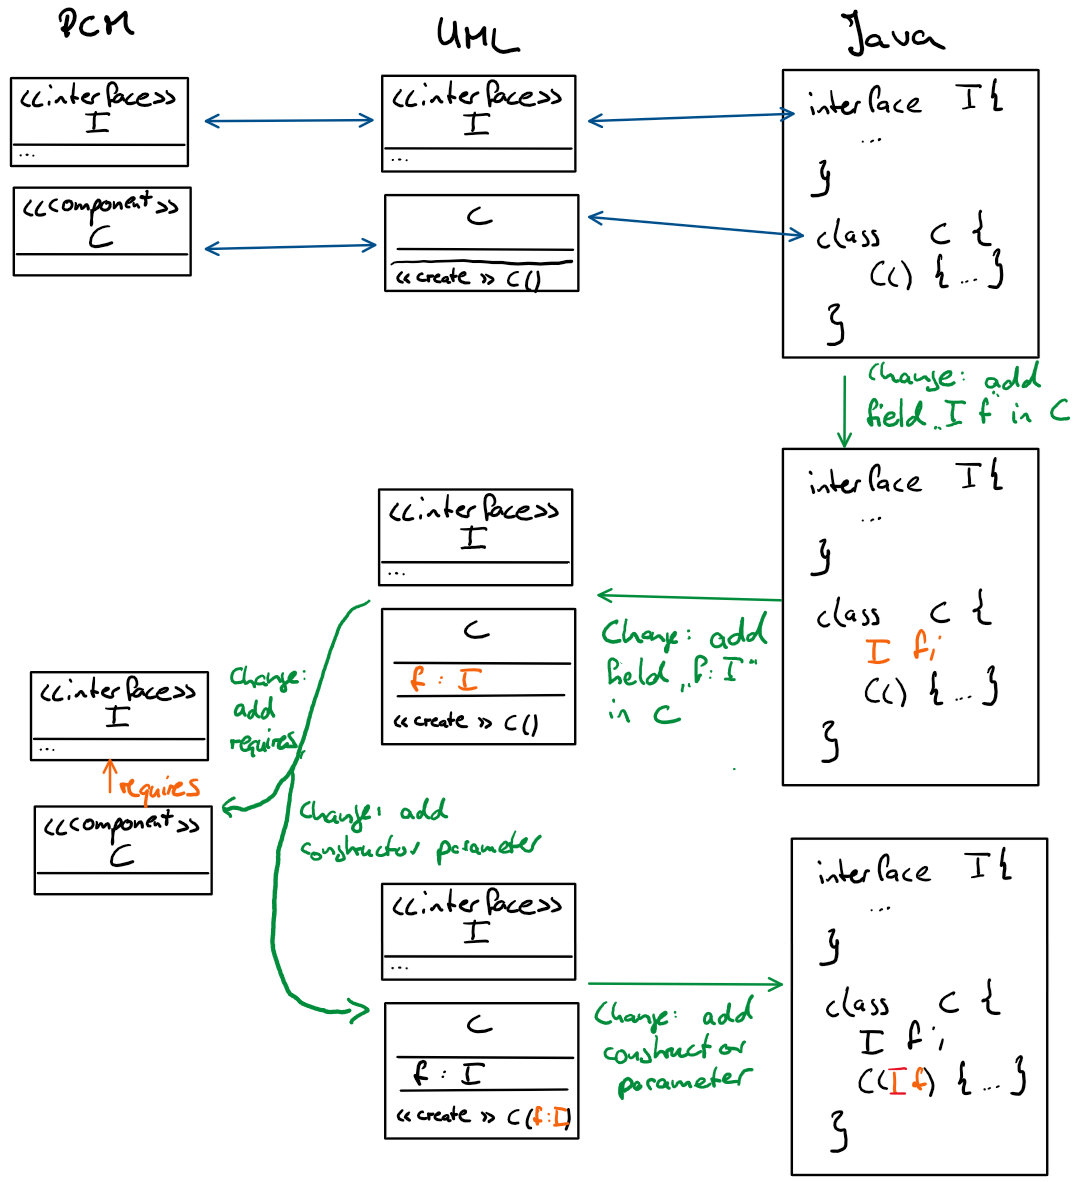
\includegraphics[width=\textwidth]{figures/correctness/orchestration/necessity_multiple_executions.png}
    \caption[Necessity of executing a transformation multiple times]{Necessity of executing a transformation multiple times. For initially consistent models, the Java code is changes, requiring \gls{UML} and \gls{PCM} models to be updated accordingly.}
    \label{fig:orchestration:necessity_multiple_executions}
\end{figure}

\mnote{Example scenario for \gls{PCM}, UML and Java}
Consider the example in \autoref{fig:orchestration:necessity_multiple_executions}, which depicts the introductory one of \autoref{fig:introduction:scenario_duplicate_execution} more precisely.
In the example, interfaces in UML and Java are related to architectural interfaces in a \gls{PCM} model.
\gls{PCM} components are realized by equally named classes in UML and Java.
Additionally, when a \gls{PCM} component requires an interface, this is realized by a field of the interface type and an appropriate constructor parameter in the component realization class in UML and Java.
Consistency is defined by transformations between \gls{PCM} and UML, as well as between UML and Java.

\mnote{Duplicate execution of transformation}
In the scenario in \autoref{fig:orchestration:necessity_multiple_executions}, we begin with a consistent state of one interface and component, each realized by an interface and class, respectively, in both UML and Java.
A user then introduces a change of the Java code, in which he or she adds a field of the interface type to the component realization class in Java.
The transformation between UML and Java propagates this change to the UML model, such that both models are consistent again.
The transformation between \gls{PCM} and UML then detects that the added field is of the type of an architectural interface, thus representing a requires relation between the corresponding component and the architectural interface. 
It adds the appropriate requires relation to the \gls{PCM} model, but also adds an appropriate parameter to the constructor of the component realization class in UML, as required by the consistency relations.
This introduces a further inconsistency between the UML and the Java model, which requires the transformation between UML and Java to be executed again to also add that constructor parameter in the Java code.

\mnote{Cycles in transformation networks}
We simplified the example to the necessary core, although in practice a further transformation between \gls{PCM} and Java would be required, for example, to ensure that the field is set within the constructor.
One might argue that having such a cycle in the graph induced by the transformations between \gls{PCM}, UML and Java could resolve the problem, as the necessary second execution of the transformation between UML and Java is not necessary if the information is propagated from \gls{PCM} to Java.
This is, however, only true if exactly that order of transformations is chosen for execution and if the transformation between \gls{PCM} and Java does not introduce further information in the Java model that then needs to be propagated to UML.

\mnote{Synchronizing transformations change already processed models}
In general, it is always possible that transformations need to react to the changes performed by others if they are not in some way aligned with each other.
This is because a synchronizing transformation may change both models.
Thus, if one transformation restores consistency between two models and another transformation reacts to that by restoring consistency between one of these models and another one, then both these models become changed, which requires the first transformation to process the newly created changes again.

\begin{figure}
    \centering
    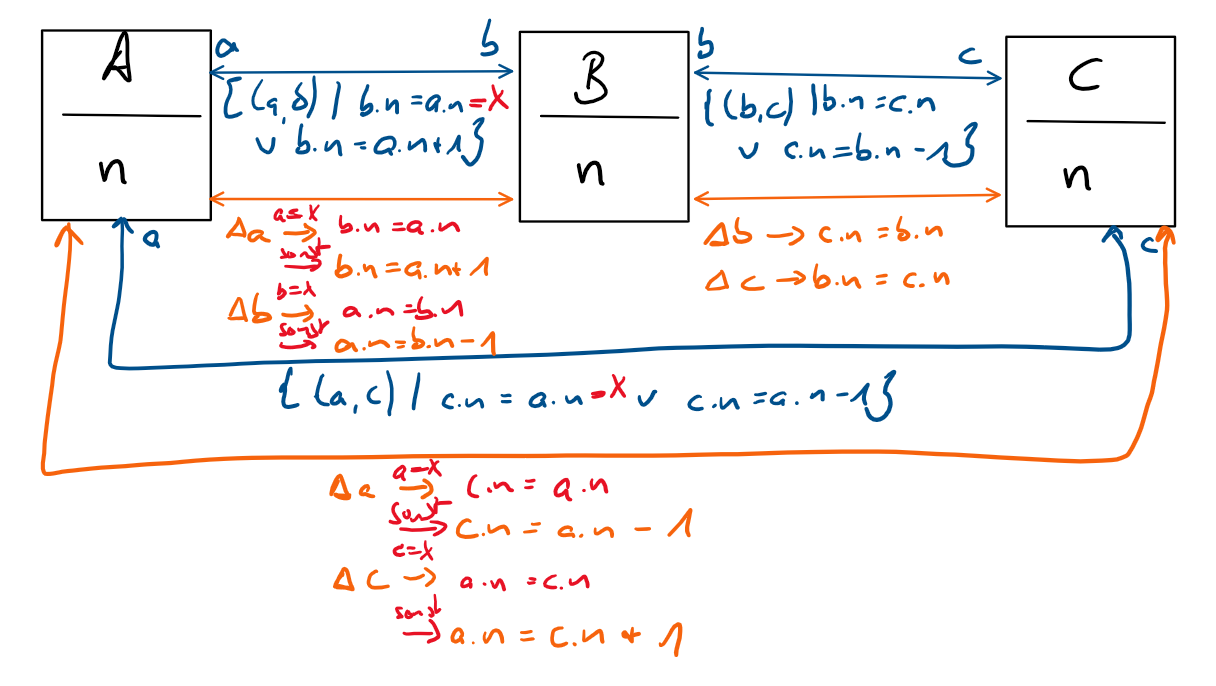
\includegraphics[width=\textwidth]{figures/correctness/orchestration/no_upper_bound_example.png}
    \caption[Example for arbitrary bounds of transformation execution]{Example for an arbitrary bound of necessary transformation execution depending on value of $x$.}
    \label{fig:orchestration:no_upper_bound}
\end{figure}

\mnote{Example generalization}
We can generalize the previous example to the one depicted in \autoref{fig:orchestration:no_upper_bound}.
It is an extension of the example given in \autoref{fig:synchronization:multiple_unidirectional_execution} for the necessity to execute the consistency preservation rules of a bidirectional transformation multiple times.
This also applies to the case in which multiple synchronizing transformations are combined.
The depicted relations and the informally defined consistency preservation rules require that elements \modelelement{A}, \modelelement{B} and \modelelement{C} with the same value of $n$ exist, and that for each \modelelement{A} with value $n$ a \modelelement{B} and \modelelement{C} with $n$ incremented by $1$ exist, except for the case that $n = x-1$.
In consequence, for an \modelelement{A} with $n = i$, all \modelelement{A}, \modelelement{B} and \modelelement{C} with $i \leq n < x$ need to exist.
This, obviously, requires the transformations to be executed $x-1-i$ times.

\mnote{Definition of example transformation network}
We prove the informally given statement with the following precise definition of the transformations for a fixed but arbitrary value of $x$.
Let $\class{A}{}, \class{B}{}, \class{C}{}$ be the classes depicted in \autoref{fig:orchestration:necessity_multiple_executions}.
\begin{align*}
    & 
    \metamodelinstanceset{M}{1} \equalsperdefinition \mathcal{P}(\instances{\class{A}{}}), %\\
    %& 
    \metamodelinstanceset{M}{2} \equalsperdefinition \mathcal{P}(\instances{\class{B}{}}), %\\
    %& 
    \metamodelinstanceset{M}{3} \equalsperdefinition \mathcal{P}(\instances{\class{C}{}}) \\[0.5em]
    &
    \consistencyrelation{CR}{12} \equalsperdefinition \setted{\tupled{a,b} \in \instances{\class{A}{}} \times \instances{\class{B}{}} \mid a.n, b.n \ge 0 \land b.n = a.n + 1 \neq x}\\
    &
    \consistencyrelationset{CR}_{12} \equalsperdefinition \setted{\consistencyrelation{CR}{12}, \consistencyrelation{CR}{12}^T} \\
    &
    \consistencypreservationrule{\consistencyrelationset{CR}_{12}}^{\rightarrow}(\model{m}{1}, \model{m}{2}, \change{\metamodel{M}{1}}) = \change{\metamodel{M}{2}} \\
    & \formulaskip
    \withmath \change{\metamodel{M}{2}}(\model{m}{2}) \equalsperdefinition \setted{b \in \instances{\class{B}{}} \mid \exists a \in \change{\metamodel{M}{1}}(\model{m}{1}) : b.n = a.n + 1 \neq x} \\
    & 
    \consistencypreservationrule{\consistencyrelationset{CR}_{12}}^{\leftarrow}(\model{m}{2}, \model{m}{1}, \change{\metamodel{M}{2}}) = \change{\metamodel{M}{1}} \\
    & \formulaskip
    \withmath \change{\metamodel{M}{1}}(\model{m}{1}) \equalsperdefinition \setted{a \in \instances{\class{A}{}} \mid \exists b \in \change{\metamodel{M}{2}}(\model{m}{2}) : b.n = a.n + 1 \neq x \land a \geq 0} \\
    &
    \transformation{t}_{12} \equalsperdefinition \tupled{\consistencyrelationset{CR}_{12}, \consistencypreservationrule{\consistencyrelationset{CR}_{12}}^{\rightarrow}, \consistencypreservationrule{\consistencyrelationset{CR}_{12}}^{\leftarrow}} \\[0.5em]
    & 
    \consistencyrelation{CR}{13} \equalsperdefinition \setted{\tupled{a,c} \in \instances{\class{A}{}} \times \instances{\class{C}{}} \mid c.n = a.n}, \consistencyrelationset{CR}_{13} \equalsperdefinition \setted{\consistencyrelation{CR}{13}, \consistencyrelation{CR}{13}^T} \\
    & 
    \consistencypreservationrule{\consistencyrelationset{CR}_{13}}^{\rightarrow}(\model{m}{1}, \model{m}{3}, \change{\metamodel{M}{1}}) = \change{\metamodel{M}{3}} \\
    & \formulaskip
    \withmath \change{\metamodel{M}{3}}(\model{m}{3}) \equalsperdefinition \setted{c \in \instances{\class{C}{}} \mid \exists a \in \change{\metamodel{M}{1}}(\model{m}{1}) : c.n = a.n} \\
    & 
    \consistencypreservationrule{\consistencyrelationset{CR}_{13}}^{\leftarrow}(\model{m}{3}, \model{m}{1}, \change{\metamodel{M}{3}}) = \change{\metamodel{M}{1}} \\
    & \formulaskip
    \withmath \change{\metamodel{M}{1}}(\model{m}{1}) \equalsperdefinition \setted{a \in \instances{\class{A}{}} \mid \exists c \in \change{\metamodel{M}{3}}(\model{m}{3}) : c.n = a.n} \\
    & 
    \transformation{t}_{13} \equalsperdefinition \tupled{\consistencyrelationset{CR}_{13}, \consistencypreservationrule{\consistencyrelationset{CR}_{13}}^{\rightarrow}, \consistencypreservationrule{\consistencyrelationset{CR}_{13}}^{\leftarrow}} \\[0.5em]
    &
    \consistencyrelation{CR}{23} \equalsperdefinition \setted{\tupled{b,c} \in \instances{\class{B}{}} \times \instances{\class{C}{}} \mid c.n = b.n}, \consistencyrelationset{CR}_{23} \equalsperdefinition \setted{\consistencyrelation{CR}{23}, \consistencyrelation{CR}{23}^T} \\
    & 
    \consistencypreservationrule{\consistencyrelationset{CR}_{23}}^{\rightarrow}, \consistencypreservationrule{\consistencyrelationset{CR}_{23}}^{\leftarrow} \andmath \transformation{t}_{23} \mathtextspacearound{accordingly} \\[1em]
    &
    \consistencyrelationset{CR} \equalsperdefinition \consistencyrelationset{CR}_{12} \cup \consistencyrelationset{CR}_{13} \cup \consistencyrelationset{CR}_{23} \\
    &
    \transformationset{T}_\mathvariable{inc} \equalsperdefinition \setted{\transformation{t}_{12}, \transformation{t}_{13}, \transformation{t}_{23}}
\end{align*}

\mnote{Minimal number of executions in example}
For these transformations, we can show that the transformation $\transformation{t}_{12}$ needs to be executed a minimal number of times depending on $x$ for a specific input.
Thus, it is not sufficient to execute each transformation only once in this network and, even worse, we can enforce the necessity for an arbitrary high number of repeated executions by proper selection of $x$.

\begin{lemma}[Minimal Number of Transformation Executions]
    \label{lemma:minimal_executions}
    Let $\transformationset{T}_\mathvariable{inc}$ be the previously defined set of transformations and let $\model{m}{1} = \model{m}{2} = \model{m}{3} = \emptyset$ be empty models and $\change{\metamodel{M}{1}} \in \changeuniverse{\metamodel{M}{1}}$ a change with $\change{\metamodel{M}{1}}(\model{m}{1}) = \setted{a \in \instances{\class{A}{}} \mid a.n = 0}$.
    Then the result of every orchestration function $\orcfunction{\transformationset{T}_\mathvariable{inc}}$ with $\appfunction{\orcfunction{\transformationset{T}_\mathvariable{inc}}}(\tupled{\model{m}{1},\model{m}{2},\model{m}{3}},\tupled{\change{\metamodel{M}{1}},\identitychange,\identitychange}) \consistenttomath \consistencyrelationset{CR}$ contains $\transformation{t}_{12}$ at least $x-1$ times.
\end{lemma}
\begin{proof}
    $\appfunction{\orcfunction{\transformationset{T}_\mathvariable{inc}}}$ can only return consistent models when it applies the transformations in the order delivered by $\orcfunction{\transformationset{T}_\mathvariable{inc}}$ by \autoref{def:applicationfunction}.
    We thus consider every orchestration, as delivered by any orchestration function, to show that it contains $\transformation{t}_{12}$ at least $x-1$ times to deliver consistent models.
    
    Let $max_n(\model{m}{1},\model{m}{2},\model{m}{3}) \equalsperdefinition max\setted{e.n \mid e \in \model{m}{1} \cup \model{m}{2} \cup \model{m}{3}}$ be the maximal value of $n$ among all instances of \modelelement{A}, \modelelement{B} and \modelelement{C} in the given models $\model{m}{1}$, $\model{m}{2}$ and $\model{m}{3}$. In the following, we shortly note $max_n$ whenever the concrete models are not relevant. We show three statements that together prove the lemma.

    \begin{properdescription}
        \item[Executing $\transformation{t}_{13}$ and $\transformation{t}_{23}$ does not increase $max_n$:]
        The transformations only ensure that for given models the returned models contain all elements with the same values of $n$ and do not introduce new elements with values of $n$ larger than the existing ones.
        \item[A single execution of $\transformation{t}_{12}$ increases $max_n$ by at most one:]
        There is no \modelelement{A} or \modelelement{B} with $n > max_n$.
        For every \modelelement{A} with $n < max_n$, $\transformation{t}_{12}$ creates, if necessary, a \modelelement{B} with value $n + 1 \leq max_n$, thus not increasing $max_n$.
        For every \modelelement{B} with $n \leq max_n$, it creates, if necessary, an \modelelement{A} with value $n-1 < max_n$.
        For every \modelelement{A} with $n = max_n$, a \modelelement{B} with value $n+1 = max_n + 1$ is created, as long as $n \neq x-1$.
        For the newly created \modelelement{B}, no further elements need to be created to fulfill the relations.
        Thus, $max_n$ is, at most, increased by $1$.
        \item[$max_n(\model{m}{1},\model{m}{2},\model{m}{3}) < x-1 \Rightarrow \tupled{\model{m}{1},\model{m}{2},\model{m}{3}} \mathtextspacearound{inconsistent to} \consistencyrelationset{CR}$:]
        There is at least one element with $n = max_n$ within the models.
        If the element with $n = max_n$ is an \modelelement{A}, there must be a \modelelement{B} with value $n+1$ due to $\consistencyrelationset{CR}_{12}$ and $n < x-1$.
        But due to $n = max_n$ such a \modelelement{B} cannot exist, because otherwise $max_n = n+1$, so this is a contradiction. 
        If the element with $n = max_n$ is a \modelelement{C}, $\consistencyrelationset{CR}_{13}$ requires an \modelelement{A} with the same value of $n$ to exist and the same argument as before leads to a contradiction.
        Finally, if the element with $n = max_n$ is a \modelelement{B}, then because of $\consistencyrelationset{CR}_{23}$ a \modelelement{C} with the same value must exist and the same argument as before leads to a contradiction.
    \end{properdescription}

    In summary, we have shown that models $\model{m}{1},\model{m}{2},\model{m}{3}$ are only consistent to $\consistencyrelationset{CR}$ when $max_n(\model{m}{1},\model{m}{2},\model{m}{3}) \geq x-1$.
    Additionally, only $\transformation{t}_{12}$ increases $max_n$ and with each execution it only increases it by at most $1$.
    In consequence, starting with $max_n = 0$, we need at least $x-1$ executions of $\transformation{t}_{12}$ in an arbitrary sequence of the transformations in $\transformationset{T}_\mathvariable{inc}$ to achieve consistent models.
\end{proof}

\mnote{Arbitrary number of necessary executions}
We have proven that arbitrary transformation networks can require an arbitrary high number of executions of each transformation.
By selecting an appropriate $x$ in the example network, we can force the network to perform at least $x-1$ executions of one transformation to yield a consistent tuple of models.
With this insight, it directly follows that we cannot find an approach to define orchestration functions that deliver sequences containing each transformation only once if we want to ensure that the approach delivers a consistent orchestration of transformations if it exists. 

\begin{theorem}[Orchestration with Single Execution]
    \label{theorem:orchestration_single}
    For a set of transformations $\transformationset{T}$, there can be models $\modeltuple{m}$ and changes $\changetuple{}$ to them for which each possible orchestration function $\orcfunction{\transformationset{T}}$ with whom $\appfunction{\orcfunction{\transformationset{T}}}(\modeltuple{m}, \changetuple{})$ is consistent, delivers a sequence as $\orcfunction{\transformationset{T}}(\modeltuple{m}, \changetuple{})$ that contains at least one transformation twice.
\end{theorem}
\begin{proof}
    According to \autoref{lemma:minimal_executions}, $\transformationset{T}_\mathvariable{inc}$ requires at least two executions of $\transformation{t}_{12}$ for the inputs in \autoref{lemma:minimal_executions} and $x \geq 3$.
    This proves the theorem by example.
\end{proof}

\mnote{Single execution insufficient}
Of course, for a concrete set of transformations it may be possible that there is an orchestration for all possible models and changes to them leading to a consistent state and only requiring each transformation to be executed once.
%We have, however, shown that this cannot be assumed in general.
\autoref{theorem:orchestration_single} shows, however, that this cannot be assumed in general.
If we execute each transformation only once, we may exclude cases for which multiple executions of transformations would have led to a consistent tuple of models.
The example we have given in \autoref{fig:orchestration:necessity_multiple_executions} is a simplification of a realistic transformation scenario, which we generalized to the previous network with transformations $\transformationset{T}_\mathvariable{inc}$.
For that reason, the insight is likely to be relevant in realistic scenarios.
We should not restrict orchestration to execute each transformation only once, as there can be realistic scenarios in which multiple executions are necessary to find consistent models.
In the following, we thus allow an arbitrary number of executions of each transformation.

\mnote{Authoritative models}
In addition, the examples, both the concrete one and the generalized abstract one, demonstrate that it can be necessary to modify the model that was originally changed by the user again.
This contradicts the notion of \emph{authoritative} models as, for example, introduced by \textcite{stevens2020BidirectionalTransformationLarge-SoSym}.
With that notion, specific models are defined authoritative and cannot be changed, for example, because they are immutable or because they were changed by the user and reverting those changes shall be avoided.
While that behavior may be a desired, forbidding the modification of a whole model to this end is not a proper solution as shown in the examples, which is why we do not consider a notion of authoritative models.


% Essential problem: One transformation may restore consistency between A and B and another between A and C. If then a transformation restores consistency between B and C, the resulting B' and C' may not be consistent A anymore.

% \todo{Beispiel warum mehrfache Ausführung nötig, warum also manche Infos erst durch andere bx reinkommen, die bei einer bx isoliert nicht relevant sind.}

% Bestehende Arbeiten (\cite{stevens2020BidirectionalTransformationLarge-SoSym}) schlagen auch vor eine Baumstruktur zu berechnen (Spannbaum), in dem nur entlang der Baumkanten die Transformationen ausgeführt werden. Dies ist jedoch eine starke Einschränkung daran, was die Transformationen ausdrücken können. Betrachtet man beispielsweise PCM, UML und Java, und hat eine Änderung in PCM. Dann könnte der Spannbaum entweder PCM -> UML -> Java sein, oder PCM -> UML + PCM -> Java. In ersterem Fall würde Verhaltensbeschreibung, die von PCM nach Java übertragen, aber in UML nicht dargestellt wird, nicht übertragen. Im zweiten Fall würde zusätzliche Information zwischen UML und Java nicht propagiert (Beispiel?) --> Hier sollte auf das Properties-Kapitel verwiesen werden, wo diese "Bottlenecks" erklärt sein sollten, inklusive einem Beispiel, die allgemein Baumstrukturen für Transformationsnetwerke ausschließen.

% Consequence: We cannot easily restrict the number of allowed executions. We can define networks that require an arbitrary number of executions.
% Also refer to the synchronization example, where we discussed that.
% Let us, for first, assume that transformations need an arbitrary number of executions.


\subsection{Orchestration Function Behavior} %The Orchestration Problem %Expected Behavior} % Failure Cases} %When to Return $\bot$?}
\label{chap:orchestration:problem:function_behavior}

\mnote{Returning $\bot$}
An application function is defined to return models only when they can be derived by applying transformations in an order delivered by the orchestration function and otherwise to return $\bot$.
In addition, we expect a \emph{correct} application function only to deliver models that are consistent.
We did, however, not yet define under which conditions we expect the function not to return $\bot$, because there are different reasons why the function may not be able to deliver consistent models although we could expect it to do so.
In fact, with the current definition, the function is even considered correct if it always returns $\bot$, which is obviously not practical.
Thus, we need to define when exactly we expect the function to return $\bot$.

\mnote{Reasons for not finding consistent orchestration}
It might be intuitive to expect an application function to always return consistent models when the input models are consistent and when there is an execution order of the transformations, i.e., an orchestration, that delivers consistent models.
This, in consequence, would lead to the requirement that the orchestration function delivers a sequence of transformations whose application delivers consistent models whenever such a sequence exists for the given models and changes to them.
There can be different reasons why the orchestration function may not deliver such a sequence:
%When is it allowed or needed to return $\bot$?
%It may always return $\bot$ to be correct, this is however not what we want.
%We can distinguish three levels of reasons why the function may not be able to find consistent models:
\begin{properdescription}
    \item[Relations are incompatible:] If the consistency relations are incompatible, a user change may introduce an element for which no consistent models exist. In consequence, the transformations cannot be executed in an order returning models that are consistent and still reflect the user change.
    %(example with employee for which no consistent other models can be found)
    \item[No consistent orchestration exists:] Even if relations are compatible, transformations may be defined in a way that they make contradictory decisions for locally consistent solutions. Thus, for a given change the consistency relations provide different ways of restoring consistency, of which each transformation selects one that is not consistent to one of the other relations.
    Then no order of the transformations can restore consistency, although consistent models exist for the given change.
    % (example with three options for name mapping with one overlapping, where each transformation always selects the one that is not appropriate for the other). We can further distinguish here whether there is always a change that cannot be processed by a CPR (then the change conflicts with the consistency relations and thus has to be rejected like any change may need to be rejected), or whether an arbitrary long sequence of transformations exists that can be applied but does never yield a consistent set of models.
    \item[No consistent orchestration found:] Finally, although an order of transformations for given changes exists that delivers consistent models, the orchestration function may not deliver it. 
    %finally, the application/orchestration may not be able to find an order of transformations that leads to a consistent state although it exists.
\end{properdescription}

\mnote{Implication hierarchy of reasons}
These reasons can be considered to reside at different levels, because each of them induces the next, i.e., if there is no orchestration, it cannot be found, and having contradictory relations, there exists no orchestration for some of the changes.
In the end, all of them lead to the situation that no orchestration can be found and, thus, the orchestration function is not able to deliver it.

\mnote{Assumption of consistent orchestration existence}
The initially given intuitive requirement that the orchestration function delivers a consistent orchestration whenever it exists would thus ensure the third level and needs to assume the first two levels to be fulfilled to avoid situations in which no consistent orchestration is found.
While we can assume compatibility of the relations, as we have discussed how to analyze it in \autoref{chap:compatibility}, we cannot assume that an orchestration does always exists, as we see in the following.

\mnote{Compatibility not ensuring consistent orchestration}
Although compatibility reduces the chance that an orchestration function does not deliver a consistent orchestration, as we have motivated with the scenario depicted in \autoref{fig:compatibility:unwanted_behavior}, it does not ensure that there is always such a sequence of transformations that the orchestration function can find.
In general, this is always the case when consistency relations define different options for consistency, i.e., they allow the existence of different corresponding elements to consider the models consistent.
Compatibility ensures that there is an overlap of these corresponding elements, such that for every element, for which consistency is restricted, consistent models can be found.
If, however, the consistency preservation rules of the transformations always restore consistency by introducing corresponding elements that are not in this overlap, each transformation will restore consistency locally to its consistency relation, but they can, together, never restore consistency to all consistency relations.

\mnote{Overlapping options in consistency relations}
Consider the situation that we have three metamodels $\metamodel{A}{}$, $\metamodel{B}{}$ and $\metamodel{C}{}$ with instances $\model{a}{i}$, $\model{b}{k}$ and $\model{c}{l}$.
Let us assume that those models are uniquely indexed by $i,k,l$ and that we defined the following \modellevelconsistencyrelations:
\begin{align*}
    &
    \consistencyrelation{CR}{AB} = \setted{\tupled{\model{a}{i}, \model{b}{k}} \mid k = i} \\
    &
    \consistencyrelation{CR}{AC} = \setted{\tupled{\model{a}{i}, \model{c}{l}} \mid l = i \lor l = i+1} \\
    &
    \consistencyrelation{CR}{BC} = \setted{\tupled{\model{b}{k}, \model{c}{l}} \mid l = k+1 \lor l = k+2}
\end{align*}
This induces the consistent model tuples $\setted{\tupled{\model{a}{i}, \model{b}{k}, \model{c}{l}} \mid  i = k = l-1}$, which are consistent to all three consistency relations.
Thus for any given model we are able to find instances of the other metamodels that are consistent to all consistency relations.
If we define consistency preservation rules for these consistency relations, the ones for $\consistencyrelation{CR}{AC}$ and $\consistencyrelation{CR}{BC}$ may decide between two models to restore consistency, because their conditions define two options for consistent models.
In the set of consistent models, however, only those models fulfilling the first of these two conditions are contained.
If the consistency preservation rules do, however, always select the models that fulfill the second condition, the resulting models are locally consistent to its consistency relation, but will never become globally consistent to all three relations.
More precisely, if the consistency preservation rules for $\consistencyrelation{CR}{AC}$ always select $\model{c}{i}$ for $\model{a}{i}$ and vice versa, and if the rules for $\consistencyrelation{CR}{BC}$ always select $\model{c}{i+2}$ for $\model{a}{i}$ and vice versa, no orchestration of the transformations will yield consistent models, because they never select those models that are in the overlap of the consistency relations.

\begin{figure}
    \centering
    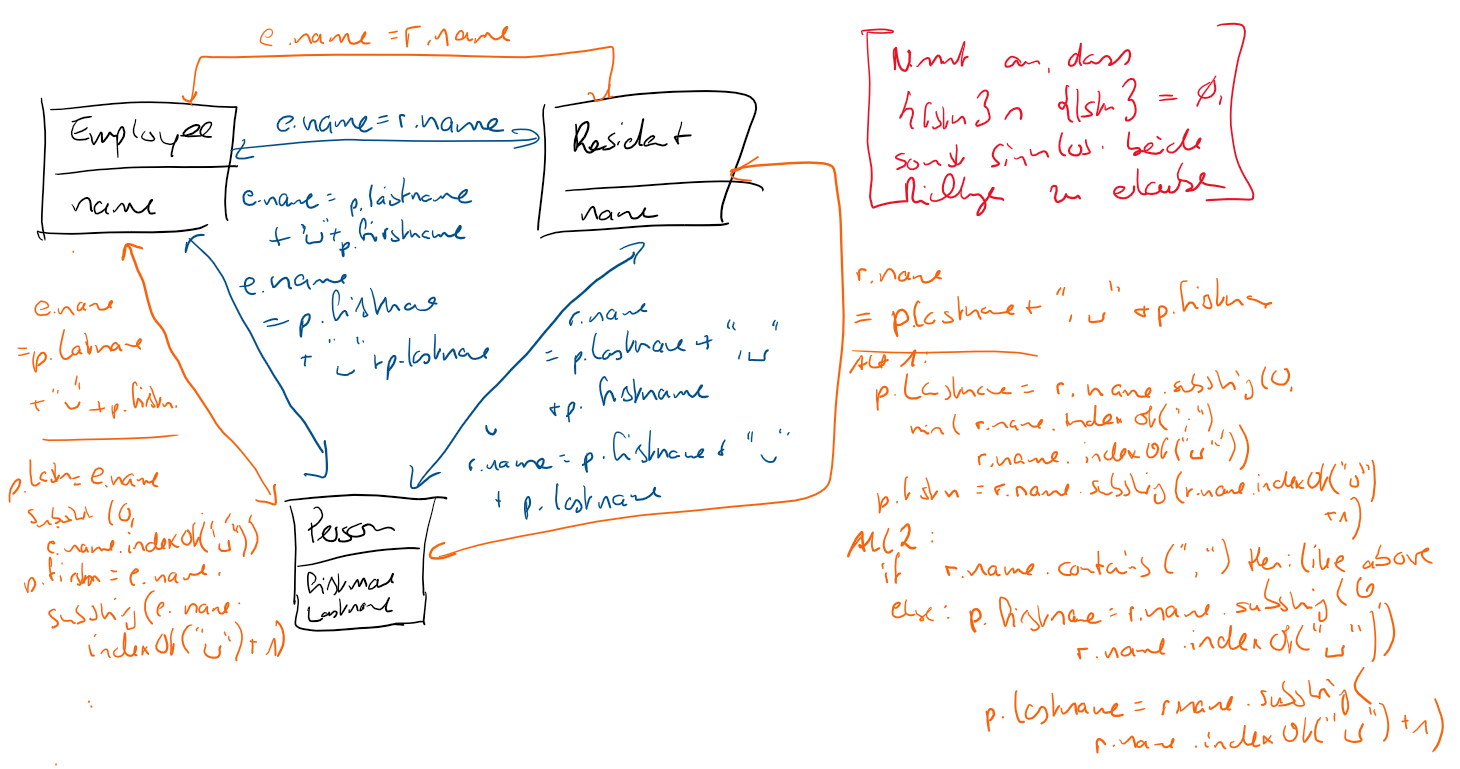
\includegraphics[width=0.85\textwidth]{figures/correctness/orchestration/no_orchestration.png}
    \caption[Consistency preservation rules without orchestration]{Consistency relations with options for corresponding elements leading to consistency preservation rules for which no consistent orchestration exists.}
    \label{fig:orchestration:no_orchestration}
\end{figure}

\mnote{Running example scenario}
%We have already given an abstract example for that problem in \autoref{fig:orchestration:no_upper_bound}. 
\autoref{fig:orchestration:no_orchestration} %, in addition, 
demonstrates this situation at a derivation of the running example.
The consistency relation between employees and residents ensures that for each resident and employee there is a corresponding other element with the same name.
The consistency relations between employees and persons and between residents and persons ensure that for each person there is a corresponding employee and resident, respectively, but they allow different relations of their names.
While both consider elements corresponding if the name of an employee and resident, respectively, are the concatenation of the first and last name of a person, an employee is also allowed to have the inverse concatenation of last and first name, whereas a resident is also allowed to have this inverse concatenation, but with an additional separation of the last and first name with a comma.
These options for the consistency relations provide further degrees of freedom for each transformation on its own, as they allow, for example, employee names to be encoded differently.
This can be reasonable if the order of first and last name is not relevant in a model managing employees.
In combination with the other consistency relations, however, the only employees, residents and persons that are considered consistent to all of the consistency relations are those having the same names with the concatenation of first and last name.
Nevertheless, these consistency relations are compatible, because for each possible condition element, i.e., for every possible employee, person and resident, there are consistent models that contain them.

\mnote{Relations without consistent orchestration}
Consistency preservation rules for these consistency relations need to choose one of the given options for the names of corresponding employees, residents and persons.
\autoref{fig:orchestration:no_orchestration} sketches consistency preservation rules that make such a selection.
The rules with alternative 1 ensure that for each employee, resident and person corresponding elements exist, which fulfill those relations of the names that are conflicting.
This means, the employee name is the concatenation of the last and first name of a person, whereas the resident name contains an additional comma in that concatenation.
In the other direction, the names of employees and residents are split at the appropriate indices, given by the whitespace and comma, respectively, to calculate the required first and last name of a person.
In consequence, there is no execution sequence of the transformations that results in consistent models, because the execution of the transformation between employees and persons always leads to a violation of the consistency relation between residents and persons and vice versa.
This is because the transformation between person and resident always introduces a comma in the resident name, which is then appended to the last name by the transformation between employee and persons.
A repeated execution of the transformation repeatedly appends that comma.
On the other hand, the execution of any of the transformations does never lead to the introduction of a person that fulfills the non-conflicting conditions of both consistency relations by simply containing a first and last name that is represented as concatenation of first and last name in both an employee and resident.
This is a concrete example for the previously discussed abstract situation that of different options in consistency relations always the non-overlapping ones are chosen by the consistency preservation rules.

\mnote{Relations with consistent orchestration}
If we consider alternative 2 for the consistency preservation rule between persons and residents, we can always find a consistent orchestration.
The alternative rule decides how consistency is ensured based on the existence of a comma within the resident name.
If a comma is present, the name relation containing a comma is used, and otherwise the simple concatenation of first and last name is assumed.
After adding an employee, first executing the transformation from employees to residents and afterwards the one from residents to persons ensures that all consistency relations are fulfilled, because the one between residents and persons sets the first and last name of a person according to the relation that is also fulfilled between person and employee, because the name does not contain a comma.
After adding a person, first executing the transformation from persons to employees and then following the process above also ensures consistency.
Finally, after adding a resident we can, for example, first apply the transformation between residents and employees and then the one between residents and persons, resulting in consistent models due to the same reasons as above.

\mnote{Only specific orchestrations are consistent}
Although consistent orchestrations of the transformations with the consistency preservation rule defined as alternative 2 exist, not every execution order leads to consistent models.
In the scenarios discussed above, we have ensured that the transformation between residents and persons is executed after the addition of a resident.
If, however, that transformation is executed after the addition of a person, a comma is added, which leads to the subsequent application of the same consistency preservation rules as with alternative 1, implying that no further orchestration yields consistent models.

\mnote{Necessity to find consistent orchestrations}
No matter whether exactly those consistency relations and preservation rules for them may occur in an actual transformation network, they exemplify the general situation of having consistency preservation rules that select one of different options provided by the consistency relations to introduce corresponding elements to restore consistency.
The example shows that whether or not a consistent orchestration of transformations exists in such a situation depends on whether at least one transformation selects an option that is consistent to other consistency relations as well.
It also shows that even if a consistent orchestration exists, not all orchestrations yield consistent models, thus we need to be able to find one that does.

\mnote{Resolvability}
In accordance with existing work \cite{stevens2020BidirectionalTransformationLarge-SoSym}, we call a given tuple of models and changes \emph{resolvable} by a transformation network, if a consistent orchestration exists.
%In contrast to existing work, we do, however, not restrict ourselves to a single execution of each transformation, as we have motivated before.
%
%\mnote{Necessity to deal with unresolvability}
We have to accept that transformation networks may be unresolvable, i.e., that there is no consistent orchestration of the transformations.
Ensuring that a network is resolvable for every change would lead to restrictions for the individual transformations that would especially require different transformations to be aligned with each other.
Since that conflicts our assumption of independent development and modular reuse, we accept unresolvability and instead focus on how we can find an orchestration if it exists. 

\mnote{Optimality property of orchestration function}
In conclusion, we expect the application function to deliver consistent models whenever a consistent orchestration, i.e., an execution order that yields consistent models, exists.
Thus, we want to ensure that the orchestration function is able to always find such an orchestration, if it exists.
We define this as an \emph{optimality} property in the following.

% "has a resolution" bei Stevens entspricht im Prinzip Kompatibilität
% "is resolvable" bei Stevens entspricht im Prinzip "orchestration exists"

% In accordance to existing work, such as \cite{stevens2020BidirectionalTransformationLarge-SoSym}, we call a given set of models and changes \emph{resolvable} by the transformation network, if there exists a sequence of the transformations such that the resulting models are consistent.
% We do, however, not restrict ourselves to a single execution of each transformation but allow them to be executed multiple times (as motivated before).
% Orchestration ermittelt eine "Resolution" (siehe bestehende Arbeiten~\cite{stevens2020BidirectionalTransformationLarge-SoSym}), also eine Ausführungsreihenfolge, zumindest wenn man sie als "korrekt" bezeichnet.

% Argumentation:
% Compatibility können wir fordern, dass eine Orchestrierungsstrategie existiert aber nicht. 

% We can avoid the first by requiring compatibility.
% We need to make restrictions to the transformation to resolve the second. We do, however, probably need to require them to know about the other transformations to avoid that. Finally, we will have to deal with that situation and then inform the user about the problem.
% We investigate whether we can always guarantee to find an orchestration if it exists.
% For now, we focus on the last problem, since that is a problem of the application and orchestration function, rather than the problem that no orchestration may exist at all.

% DECIDED THAT THE FOLLOWING IS NOT AN OPTION BUT THE SECOND IS DEFINITE.
% Now we have these options:
% \begin{itemize}
%     \item We accept that there is no orchestration or that the strategy does not find it in specific situations, than we only need to consider that the strategy must always terminate.
%     We could, for example, change the algorithm such that it always returns $\bot$, which is correct, or terminates after executing each transformation once.
%     \item We define a precise criterion when the strategy is allowed to return $\bot$. Most intuitively, one might say that it should only return $\bot$ whenever no orchestration exists.
% \end{itemize}



\subsection{Optimal Orchestration}

% An application function that delivers consistent models whenever an orchestration exists that yields them is what we would assume \emph{optimal}.
% Recall that $\generalizationfunction{\metamodeltuple{M},\transformation{t}}$ is the generalization function that applies a transformation, which is only defined for two models, to a model tuple that instantiate all metamodels in $\metamodeltuple{M}$.

% \begin{definition}[Optimal Transformation Application Function]
%     Let $\transformationset{T}$ be a set of transformations for a set of metamodels $\metamodeltuple{M} = \tupled{\metamodelsequence{M}{n}}$.
%     We say that an application function $\appfunction{\orcfunction{\transformationset{T}}}$ for these transformations is \emph{optimal} if it returns models that are consistent whenever there is an orchestration of the transformation that yields a consistent set of models whenever it exists, i.e.,
%     \begin{align*}
%         &
%         \forall \modeltuple{m} \in \metamodeltupleinstanceset{M} : \forall \changetuple{\metamodeltuple{M}} = \tupled{\change{\metamodel{M}{1}}, \dots, \change{\metamodel{M}{n}}} \in \changeuniverse{\metamodeltuple{M}} :
%         \modeltuple{m} \consistenttomath \consistencyrelationset{CR} \Rightarrow \\
%         & \formulaskip
%         \bigl(
%             \exists \transformation{t}_{1}, \dots, \transformation{t}_{m} \in \transformationset{} : 
%             \exists \changetuple{\metamodeltuple{M}}' = \tupled{\change{\metamodel{M}{1}}', \dots, \change{\metamodel{M}{n}}'} \in \changeuniverse{\metamodeltuple{M}} :\\
%             & \formulaskip \formulaskip
%             \generalizationfunction{\metamodeltuple{M}, \transformation{t}_{1}} \concatfunction \dots \concatfunction \generalizationfunction{\metamodeltuple{M}, \transformation{t}_{m}}(\modeltuple{m}, \changetuple{\metamodeltuple{M}}) = (\modeltuple{m}, \changetuple{\metamodeltuple{M}}')\\
%             & \formulaskip \formulaskip
%             \land \tupled{\change{\metamodel{M}{1}}'(\model{m}{1}), \dots, \change{\metamodel{M}{n}}'(\model{m}{n})} \consistenttomath \consistencyrelationset{CR} \bigr) \\
%             & \formulaskip
%             \Rightarrow \appfunction{\orcfunction{\transformationset{T}}}(\modeltuple{m},\changetuple{\metamodeltuple{M}}) \consistenttomath \consistencyrelationset{CR}
%         \bigr)
%     \end{align*}
% \end{definition}

\mnote{Optimal orchestration function}
To ensure that an application function delivers consistent models whenever a consistent orchestration exists, we need to find an orchestration function that fulfills this property.
We denote this as an \emph{optimal} orchestration function.
Recall that $\generalizationfunction{\metamodeltuple{M},\transformation{t}}$ is the generalization function that applies a transformation, which is only defined for two models, to a model tuple that instantiate all metamodels in $\metamodeltuple{M}$.
% It is obvious that we can define consistency preservation rules for which the orchestration function cannot find an execution order that returns a consistent tuple of models after certain changes. We already gave an example in \autoref{fig:correctness:no_execution_order}. There exists no execution order for any input value that terminates. The transformations will always increase the value, although the defined relations could be fulfilled for the input value, but the transformations never find that solution.

% Although we will discuss restrictions to relations and transformations that reduce the chance that no solution can be found, it will not be possible to ensure that such a solution can always be found. This is due to the reason that transformations can perform arbitrary changes given that transformations are Turing complete, which should not be restricted, because it is unclear which restrictions could be made without forbidding scenarios that should actually we supported. Thus, we assume that transformations are Turing complete.

% We explicitly allow the orchestration function to return a sequence that will, if applied to models and changes to them, not deliver a consistent tuple of models. As discusses, this is supposed to reflect cases in which no such sequence can be calculated.
% However, it may be useful to have some notion of \emph{optimality} that ensures that if a sequence that delivers a consistent result exists, the orchestration function is supposed to find it.
% Formally, this notion looks as follows.

\begin{definition}[Optimal Orchestration Function]
    Let $\transformationset{T}$ be a set of transformations for a metamodel tuple $\metamodeltuple{M}% = \tupled{\metamodelsequence{M}{n}}
    $.
    We say that an orchestration function $\orcfunction{\transformationset{T}}$ for these transformations is \emph{optimal} if, and only if, it returns a consistent orchestration whenever it exists:
    \begin{align*}
        &
        \forall \modeltuple{m} \in \setted{\modeltuple{m}' \in \metamodeltupleinstanceset{M} \mid \modeltuple{m}' \consistenttomath \consistencyrelationset{CR}} : \forall \changetuple{\metamodeltuple{M}} %= \tupled{\change{\metamodel{M}{1}}, \dots, \change{\metamodel{M}{n}}} 
        \in \changeuniverse{\metamodeltuple{M}} : \\
        %\modeltuple{m} \consistenttomath \consistencyrelationset{CR} \Rightarrow \\
        & \formulaskip
        %\bigl[ 
            \bigl(
            \exists \transformation{t}_{1}, \dots, \transformation{t}_{i} \in \transformationset{T} : 
            \exists \changetuple{\metamodeltuple{M}}' %= \tupled{\change{\metamodel{M}{1}}', \dots, \change{\metamodel{M}{n}}'} 
            \in \changeuniverse{\metamodeltuple{M}} : \changetuple{\metamodeltuple{M}}'(\modeltuple{m})
            \consistenttomath \consistencyrelationset{CR}\\
            & \formulaskip \formulaskip
            \land \generalizationfunction{\metamodeltuple{M}, \transformation{t}_{i}} \concatfunction \dots \concatfunction \generalizationfunction{\metamodeltuple{M}, \transformation{t}_{1}}(\modeltuple{m}, \changetuple{\metamodeltuple{M}}) = (\modeltuple{m}, \changetuple{\metamodeltuple{M}}')
            \\
            % & \formulaskip \formulaskip
            %\land \changetuple{\metamodeltuple{M}}'(\modeltuple{m})
            %\tupled{\change{\metamodel{M}{1}}'(\model{m}{1}), \dots, \change{\metamodel{M}{n}}'(\model{m}{n})} 
            %\consistenttomath \consistencyrelationset{CR} \bigr) \\
            & \formulaskip
            \Rightarrow
            \exists \transformation{t}_{1}', \dots, \transformation{t}_{k}' \in \transformationset{T} : 
            \exists \changetuple{\metamodeltuple{M}}'' %= \tupled{\change{\metamodel{M}{1}}'', \dots, \change{\metamodel{M}{n}}''} 
            \in \changeuniverse{\metamodeltuple{M}} : \changetuple{\metamodeltuple{M}}''(\modeltuple{m}) \consistenttomath \consistencyrelationset{CR}\\
            & \formulaskip \formulaskip
            \land \generalizationfunction{\metamodeltuple{M},\transformation{t}_{k}'} \concatfunction \dots \concatfunction \generalizationfunction{\metamodeltuple{M},\transformation{t}_{1}'}(\modeltuple{m}, \changetuple{\metamodeltuple{M}}) = (\modeltuple{m}, \changetuple{\metamodeltuple{M}}'') \\
            & \formulaskip \formulaskip
            \land \orcfunction{\transformationset{T}}(\modeltuple{m}, \changetuple{\metamodeltuple{M}}) = \sequenced{\transformation{t}_{1}', \dots, \transformation{t}_{k}'} %\\
            % & \formulaskip \formulaskip
            % \land \changetuple{\metamodeltuple{M}}''(\modeltuple{m})
            % %\tupled{\change{\metamodel{M}{1}}''(\model{m}{1}), \dots, \change{\metamodel{M}{n}}''(\model{m}{n})} 
            % \consistenttomath \consistencyrelationset{CR}
        \bigr) %\bigr]
    \end{align*}
\end{definition}

\mnote{Behavior without consistent orchestration existence}
Note that we allow an optimal orchestration function to return a sequence even when there is no consistent orchestration.
This is reasonable, because an application function may be defined to return consistent models whenever there is a consistent orchestration, but to also to support the process of identifying why there is no such order by delivering a sequence of transformations that leads to a failure, as we will discuss in \autoref{chap:orchestration:algorithm}.

\mnote{Application function optimality}
Finally, the result of the application function is what is relevant in the process of consistency preservation in a transformation network.
Thus, we apply the notion of \emph{optimality} to that function accordingly by requiring it to deliver consistent models whenever a consistent orchestration exists.

\begin{definition}[Optimal Application Function]
    \label{def:optimalapplicationfunction}
    Let $\transformationset{T}$ be a set of transformations for a tuple of metamodels $\metamodeltuple{M} %= \tupled{\metamodelsequence{M}{n}}
    $.
    We say that an application function $\appfunction{\orcfunction{\transformationset{T}}}$ for these transformations is \emph{optimal} if, and only if, it returns models that are consistent whenever there is a consistent orchestration of the transformations:
    \begin{align*}
        &
        \forall \modeltuple{m} \in \setted{\modeltuple{m}' \in \metamodeltupleinstanceset{M} \mid \modeltuple{m}' \consistenttomath \consistencyrelationset{CR}} : \forall \changetuple{\metamodeltuple{M}} %= \tupled{\change{\metamodel{M}{1}}, \dots, \change{\metamodel{M}{n}}} 
        \in \changeuniverse{\metamodeltuple{M}} : \\
        %\modeltuple{m} \consistenttomath \consistencyrelationset{CR} \Rightarrow \\
        & \formulaskip
        \bigl(
            \exists \transformation{t}_{1}, \dots, \transformation{t}_{m} \in \transformationset{T} : 
            \exists \changetuple{\metamodeltuple{M}}' %= \tupled{\change{\metamodel{M}{1}}', \dots, \change{\metamodel{M}{n}}'} 
            \in \changeuniverse{\metamodeltuple{M}} : \changetuple{\metamodeltuple{M}}'(\modeltuple{m}) \consistenttomath \consistencyrelationset{CR}\\
            & \formulaskip \formulaskip
            \land \generalizationfunction{\metamodeltuple{M}, \transformation{t}_{1}} \concatfunction \dots \concatfunction \generalizationfunction{\metamodeltuple{M}, \transformation{t}_{m}}(\modeltuple{m}, \changetuple{\metamodeltuple{M}}) = (\modeltuple{m}, \changetuple{\metamodeltuple{M}}') %\\
            %& \formulaskip \formulaskip
            %\land \tupled{\change{\metamodel{M}{1}}'(\model{m}{1}), \dots, \change{\metamodel{M}{n}}'(\model{m}{n})} \consistenttomath \consistencyrelationset{CR} 
            %\bigr) 
            \\
            & \formulaskip
            \Rightarrow \appfunction{\orcfunction{\transformationset{T}}}(\modeltuple{m},\changetuple{\metamodeltuple{M}}) \consistenttomath \consistencyrelationset{CR}
        \bigr)
    \end{align*}
\end{definition}

\mnote{Optimality dependency}
According to the defined behavior of an application function, an optimal application function requires an optimal orchestration function.

\begin{lemma}[Application / Orchestration Function Optimality]
    \label{lemma:optimalapplicationfunction}
    An application function $\appfunction{\orcfunction{\transformationset{T}}}$ can only be optimal if $\orcfunction{\transformationset{T}}$ is optimal.
\end{lemma}
\begin{proof}
    Let us assume that the complete condition in \autoref{def:optimalapplicationfunction} is fulfilled, i.e., that the input models are consistent and that a consistent orchestration of the transformations exists for the given models and changes.
    Then, to be optimal, the application function needs to return models that are consistent.
    According to the definition of an application function (see \autoref{def:applicationfunction}), the sequence of transformations delivered by $\orcfunction{\transformationset{T}}$ for that input must yield the same model tuple as $\appfunction{\orcfunction{\transformationset{T}}}$.
    Thus, the orchestration function must deliver a sequence for such inputs that yields consistent models, which is equivalent to $\orcfunction{\transformationset{T}}$ being optimal.
\end{proof}


\subsection{The Orchestration Problem}

\mnote{Orchestration problem}
The problem to find a consistent orchestration whenever it is exists, i.e., to find an optimal orchestration function, is the central subject of the following sections.
This is what we denote as the \emph{orchestration problem}.
We prove that the problem is undecidable, discuss how we can make it decidable and propose strategies to deal with its undecidability.
Finally, we come up with a discussion of conservatively approximating a solution to the problem.
We define the problem as follows.
\begin{definition}[Orchestration Problem]
    \label{def:orchestrationproblem}
    The problem to find a consistent orchestration of transformations for given inputs (models and changes to them) if it exists is called the orchestration problem.
\end{definition}

\mnote{Orchestration existence problem}
Often, the more general problem of deciding whether a consistent orchestration exists is sufficient for us.
\begin{definition}[Orchestration Existence Problem]
    \label{def:orchestrationexistenceproblem}
    The question whether a consistent orchestration of transformations for given inputs (models and changes to them) exists is called the orchestration existence problem.
\end{definition}

\mnote{Problem equivalence}
In fact, both these problems are equivalent in the sense that having a solution for one of them also delivers a solution for the other.
\begin{theorem}[Orchestration / Existence Problem Equivalence]
    \label{theorem:orchestrationproblemequivalence}
    The orchestration problem can be solved if, and only if, the orchestration existence problem can be solved.
\end{theorem}
\begin{proof}
    If a solution for the orchestration problem exists, it directly induces a solution for the orchestration existence problem, because if we find a consistent orchestration whenever it exists, we also know whether it exists.
    If a solution for the orchestration existence problem exists and we know that a consistent orchestration exists, we can find it by systematically testing all orchestrations of growing size until a consistent orchestration is found. Since we know that such an orchestration exists, this test must terminate, even if it may take an impractically long time.
\end{proof}

\mnote{Problem to optimality equivalence}
Since the orchestration problem is derived from the goal of finding an optimal application function, it is obviously equivalent to find an optimal application function or to solve the orchestration (existence) problem.
%As both problems are equivalent, we prove this for the orchestration existence problem.

\begin{theorem}[Optimality / Orchestration Problem Equivalence]
    \label{theorem:optimal_application_function_orchestration_problem}
    An optimal application function $\appfunction{\orcfunction{\transformationset{T}}}$ can be defined if, and only if, a solution for the orchestration (existence) problem exists.
\end{theorem}
\begin{proof}
    We give the proof for the orchestration existence problem, which is, according to \autoref{theorem:orchestrationproblemequivalence} equivalent to the orchestration problem.
    An optimal $\appfunction{\orcfunction{\transformationset{T}}}$ returns consistent models whenever there is a consistent orchestration.
    With such a function, we are able to decide whether such an orchestration exists or not.
    \begin{align*}
        \function{ExistsOrc}(\transformationset{T},\modeltuple{m},\changetuple{\metamodeltuple{M}}) \equalsperdefinition
            \begin{cases}
                \textsc{true}, & \appfunction{\orcfunction{\transformationset{T}}}(\modeltuple{m},\changetuple{\metamodeltuple{M}}) \consistenttomath \transformationset{T} \\
                \textsc{false}, & otherwise
            \end{cases}
    \end{align*}
    $\function{ExistsOrc}$ returns \textsc{true} if, and only if, a consistent orchestration exists.
    $\appfunction{\orcfunction{\transformationset{T}}}$ does, per definition, only return consistent models when there is an orchestration that yields them.
    Since it is optimal, it does always return consistent models when an orchestration that yields them exists.
\end{proof}

